\chapter{Implementation}\label{ch:impl}

In this chapter, we discuss the implementation of the individual components
presented in the previous chapter, but we also present some shared implementation
features, such as the common request/response protocol used for the
communication between the different components.

\section{Coordinator}

As the central component of our system, the coordinator performs a rich
set of tasks. These involve handling submission requests to spawn new queries,
but also handling publication and subscription requests from existing queries.
It is the central authority about the current system state, i.e. it maintains
a list of all running queries and executors, but it also tracks all existing
publications and subscriptions. It exposes this information in the catalog.

Because most components interact with the coordinator, its
internal implementation is not without challenges. The two major ones
being the fact that it has to deal with many concurrent asynchronous events,
and secondly that it has to maintain shared mutable state.

Before we discuss these challenges, we provide a brief overview over the
internal architecture of the coordinator: To other components, the coordinator
exposes a request/response-based interface on a predefined networking port.
For this purpose, the coordinator listens for incoming connections on that port
and then waits for the connected clients to send requests. Once requests are
received and decoded, they are forwarded to a central request handler. This
request handler contains the central logic of the coordinator, keeps track of
unfulfilled requests and mutates the catalog to announce changes in the
system state.

\paragraph{Dealing with asynchronous events}
The initial prototype of the coordinator used a multi-threaded approach for dealing
with multiple clients at the same time, and used message passing between threads
to avoid directly exposing shared state. However, many requests handled by
the coordinator require it to wait for external events, and thus a form of
cooperative task management is needed.

We initially used a continuation-passing style for splitting blocking requests into
non-blocking subtasks. However, due to Rust's memory ownership model, we found that
this approach often resulted in manual \emph{stack ripping} \cite{stackmgmt},
which made code both hard to read and inconvenient to write.

This motivated us to re-design the coordinator around a central event loop, which
allows us to multiplex many asynchronous tasks within the same thread. However,
instead of using callbacks as event handlers, we decided to adapt an external
library called \lstinline{future-rs} \cite{futuresrs}. It provides a more expressive interface
for dealing with asynchronous tasks based on the concept of \emph{futures}. Futures
(sometimes called promises, eventuals or deferred objects) are proxy objects for
values that will eventually will be provided through some asynchronous event.
The \lstinline{future-rs} library provides combinators for chaining events
together or waiting on multiple events at the same time. The library itself
only provides an abstract interface for dealing with futures, the actual
dispatching of events has to be implemented externally, which we did in the
aforementioned event loop.

With this abstraction, requests that might be completed asynchronously
(i.e. a blocking subscription request for a topic which has not yet been registered)
are split up into a future representing the pending response, and a completion handle
which is invoked once the request can be resolved. Bookkeeping of pending requests
is done in the request handler.

\paragraph{Maintaining shared mutable state}

The nature of the coordinator requires it to mutate its internal state on
behalf of the connected clients. As the Rust programming language discourages
the use of aliased directly mutable references, we have to provide a wrapper
type which allows the connection handlers mutable access to the request handler.

Because all requests originating from a certain connection are issued using a
wrapper, we can use it to keep track of the requests submitted by that connection.
This allows us to clean up any associated state if the connection disappears,
such as removing disconnected executors from the pool, or depublishing 
topics of crashed workers.

\subsection{Catalog}

The purpose of the catalog is to maintain and expose the current state of the
system. It tracks the addition or removal of executors, queries, topics,
publication and subscriptions and exposes them in collection topics according
to the schema shown in Figure~\ref{fig:model}.

\begin{figure}[htb]
  \centering
    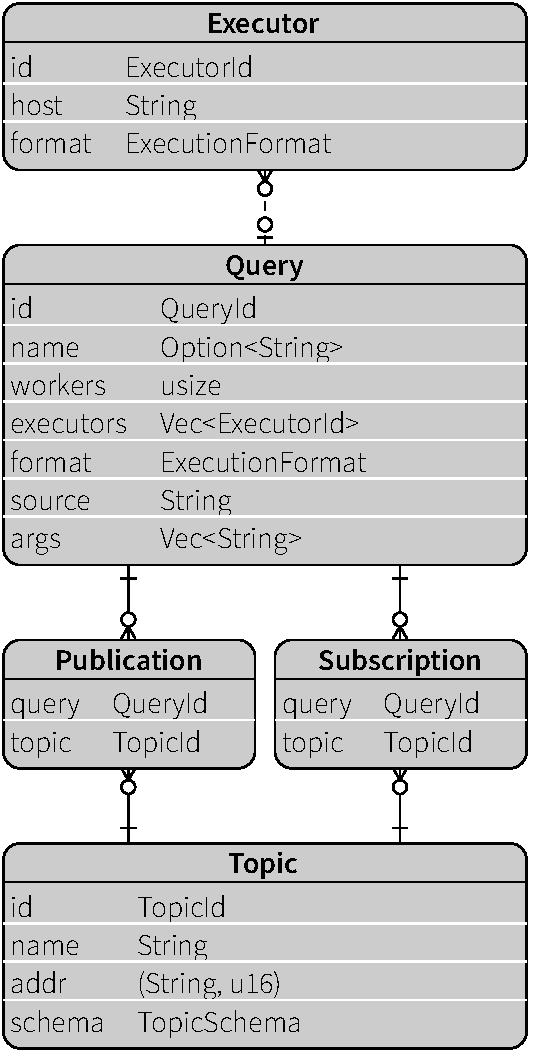
\includegraphics[width=0.5\textwidth]{figures/model}
  \caption[Schema of the catalog.]{Schema of the catalog. All five data types
  are published as a collection topic, allowing users to follow state changes
  in the system.}
  \label{fig:model}
\end{figure}

The catalog itself only exposes this data. It is mutated and queried by the
request handler in order fulfill certain requests.

\section{Executor}

The current implementation of the executor is relatively simple. It is an executable
that registers itself at the coordinator and then spawns child processes on behalf
of the coordinator.

In order to add a new host to the cluster, the user has to deploy the executor
binary on the new host, specify the address of the coordinator and then launch
the executor binary. The executor registers itself at the coordinator, which
assigns a unique identifier to the connecting executor. Once connected to the
coordinator, the executor listens for incoming spawn requests. If such an
request arrives, it fetches the binary from the specified source and launches
it as an operating system process. Any command line arguments to be passed
to the query are provided here as well.

The executor has to inform the spawned binary about its assigned query identify,
the address of the coordinator and the address of any peer processes. In the
current implementation this is simply done using environment variables, which
can easily be accessed by the spawned query.

% TODO talk about supported url formats
% TODO talk about stdout forwarding

\section{Query Library}

We provide a small wrapper library which allows Timely processes to participate
in our system. A query submitted to the system must eventually call the 
\lstinline{timely_query::execute} function, a function which mirrors Timely's
own \lstinline{execute} function. When called, this function parses the
environment variables mentioned above which are provided by the executor.
Using this information, the process connects to the coordinator and registers
itself by providing its identifer and the group of workers it will host. Once
all worker groups have successfully registered themselves at the coordinator,
the coordinator replies with a randomized token which is used to identify
the registered processes belonging to a query. 

The initialization of the Timely worker threads and the allocation of the
communication channels among then is done using \lstinline{time\-ly_\-com\-mu\-ni\-ca\-tion}
the same way as it would be done in a standalone Timely program. For this
reason, our query library needs to translate the information provided by the
executor into Timely's own format.

Our query library also needs to provide an interface for worker threads to
publish or subscribe to topics. For this reason, every worker thread gets
a handle for the connection to the coordinator. Access to the
publish \& subscribe system is provided through a set of remote
procedure call stubs which are described in the following section.

\subsection{Publishers \& Subscribers}

The query library exposes the publish and subscribe functionality. The following
API is used for publishing and subscribing to Timely streams.

\begin{lstlisting}[caption={[Publish \& subscribe interface]
The interface for publishing and subscribing Timely streams.
}]
pub struct Coordinator {
  /* hidden handle to request queue */
}

impl Coordinator {
  pub fn publish<S, D>(&self, name: &str, stream: &Stream<S, D>,
    partition: Partition) -> Result<Stream<S, D>, PublicationError>
      where D: Data + NonStatic, 
            S: Scope,
            S::Timestamp: NonStatic;

  pub fn subscribe<T, D>(&self, name: &str, cap: Capability<T>) 
    -> Result<TimelySubscription<T, D>, SubscriptionError>
      where T: Timestamp + NonStatic, 
            D: Data + NonStatic;
}
\end{lstlisting}

The \lstinline{NonStatic} bounds on the data and timestamp
parameters are required for safe serialization described in \ref{sec:serialization}.

\subsubsection{Publisher}

The \lstinline{publish} function takes a direct reference to a Timely
\lstinline{Stream<S, D>}. These stream handles, which are only available during
the dataflow graph construction phase, allow us to instantiate our own publish
operator on the stream.  The instantiated publish operator will push both, its
incoming data, as well as its current frontier to any subscribers. 

Once the operator is inserted into the dataflow graph, the \lstinline{publish}
stub issues a registration request to the coordinator, which will result in the
creation of a topic for other queries to subscribe to.

The \lstinline{partition} argument on the API specifies whether all streams
shall be merged into a single topic, of if every worker publishes its own stream.
In the second case, the identifier of the publishing worker is appended to the
name of the topic:

\begin{lstlisting}[caption={
Example use of publisher.
}]
timely_query::execute(|root, coord| {
    root.scoped::<u64, _, _>(|scope| {
        let i = scope.index();
        let numbers = (i*100..(i+1)*100).to_stream(scope);

        // results in `n` topics:
        //    "numbers.0", "numbers.1", .., "numbers.n"
        coord.publish("numbers", &numbers, Partition::PerWorker)
             .expect("failed to publish topic");

        // filtering performed by each worker in parallel
        let primes = numbers.filter(|x| x.is_prime());

        // results in a single merged topic called "primes",
        // published by worker number 0
        coord.publish("primes", &primes, Partition::Merge)
             .expect("failed to publish topic");
    });
})
\end{lstlisting}


\paragraph{Collection Publisher}

In addition to the stream publisher, we also provide the so called collection
publisher. It has a similar interface for publishing, but it requires the
type of the incoming stream to deliver \lstinline{(D, i32)} tuples, where
the integer denotes the amount of elements have been added or removed from
the collection.

\begin{lstlisting}[caption={[Collection publisher interface]
}]
impl Coordinator {
  pub fn publish_collection<S, D>(&self, name: &str,
    stream: &Stream<S, (D, i32)>, partition: Partition)
    -> Result<Stream<S, (D, i32)>, PublicationError>
      where D: Data + NonStatic, 
            S: Scope,
            S::Timestamp: NonStatic;
}
\end{lstlisting}

Internally, the publisher maintains a copy of this collection. This is required
for new subscribers, which must be informed about the contents of the collection
when they connect.

\paragraph{Implementation Details}

Both publishers share the same underlying logic which accepts incoming connections
from subscribers and provides a notifications for disconnected clients.

Internally, this logic also make use of the \lstinline{future-rs} library, 
since futures have also been integrated in our networking layer. A unique
aspect of the futures provided by \lstinline{future-rs} is that they need
be polled in order to make progress.

Inside the coordinator the polling is done by its event loop. For the futures
inside our publish and subscribe operators however we make use of the fact
that Timely itself also uses polling-based scheduling. This guarantees that
the surrounding Timely operator is polled regularly, enabling it to poll
the contained futures for completion.

\subsubsection{Subscriber}

In contrast to the publisher, the current implementation of the \lstinline{subscribe}
function does not directly instantiate a Timely operator, but returns a subscription
handle which is used to read data from the topic.

There are two reasons for this choice: First, Timely requires that an operator
is instantiated on every worker. It can happen that the amount of topics a query
would like to subscribe to and the amount of workers do not match. Thus, the API
quickly becomes complicated, as we would need to provide an interface assigning
topics to operators.
Second, Timely's operator contract requires that an operator instance announces
the internal initial capabilities it holds, and, more importantly, the initial
capabilities of its peers. To support this would require some synchronization
between the subscribers, as they have to exchange the initial frontier they
observe at their topic.

Instead, we decided to base our subscription progress tracking on Timely's new
capability handles. The recently added \emph{unordered input operator} allows
a query to feed a computation from data with unordered timestamps. This operator
exposes a root capability for the earliest possible timestamp, allowing the user
to derive capabilities for newer timestamps from old ones. The frontier
is advanced by dropping the capabilities for timestamps for which no more data
is pending.

Based on the progress tracking information delivered by the publisher, the
subscription handle will automatically derive new capabilities for incoming
data and drop old ones if the frontier advances. The user however has to
provide the initial root capability for the input.

\begin{lstlisting}[caption={[Typical use of the subscription handle]
Typical use of the subscription handle. This query subscribes to a single topic of
strings, with \lstinline{u64} being the type of the timestamps.
}]
timely_query::execute(|root, coord| {

    let (mut input, cap) = root.scoped::<u64, _, _>(|scope| {
        let ((input, cap), stream) = scope.new_unordered_input();
        // stream.operators(..)
        (input, cap)
    });

    let topic = coord.subscribe::<_, String>("example", cap)
                     .expect("failed to subscribe");

    for (time, data) in topic {
        let session = input.session(time);
        session.give_content(&mut Content::Typed(data));
        root.step();
    }
})
\end{lstlisting}

In queries which use multiple workers, the query author can decide which workers
actually subscribe to topics, as the code outside the graph generation is allowed
to conditionally decide if it wants to call the subscribe function. Because
the root capability can be cloned, this interface also allows the user to
interleave the data from a topic with other data, for example by merging
multiple topics at the input.

\section{Shared Communications Layer}

For the remainder of this chapter we discuss the networking and communications
layer of our system, which is used all components for implementing their
services.

\subsection{Messaging}

Our system consists of potentially many distributed processes. These processes
are running concurrently, are dynamically added and removed from the system
and are communicating with each other. In order to deal with the inherent
complexity of such a system, we adopted an actor-model like approach for our
implementation.

Actors in our system include processes like the coordinator, the executors 
and the query processes. However, as Timely by itself could be seen as an
actor system, operators like the publish or subscribe operators are also actors
directly interacting with our system.

To support this kind of model, our networking layer also works in terms of
asynchronous messages. In contrast to Timely's own networking layer which also
provides a similar abstraction, we cannot assume a fixed number of actors.
In order to establish a connection between two components, one of them has to
take on the role of the server, while the other one acts as a client. Two
queues are allocated per connection on each actor: one for incoming messages
and one for outgoing messages. This enables messages to be sent asynchronously
in both directions. Network failures are signaled in the queue for incoming
messages. Currently, Rust's standard library TCP sockets are used as the
underlying transport mechanism, however the system could easily be extended to
support alternative transport layers as well.

\subsection{Request \& Response Messages} \label{sec:reqresp}

While the abstraction of single messages is sufficient for implementing the
mostly unidirectional messaging paradigm of the publish-subscribe implementation,
most other communication in the system follows a request-response pattern.
For this reason, we implemented a request-response multiplexer on
top of the plain message channels. This multiplexer allows both actors to have
multiple requests in flight while waiting for the corresponding responses,
which can be delivered out of order.

In order to differentiate between different kind of requests and also ensure a
well-typed response format, request payloads have to implement the \lstinline{Request}
trait. The associated name is used for decoding, while the associated \lstinline{Success}
and \lstinline{Error} types specify what kind of payloads are valid for the response.
This allows the response for a given request \lstinline{R} to be represented by
Rust's \lstinline{Result<R::Success, R::Error>} type.

\begin{lstlisting}[caption={[Request trait]In order for a type to be used as a
request message, it needs to implement the \lstinline{Request} trait. The name allows
request handlers to differentiate between different types of requests, while the associated
types forces them to issue well-formed responses.
The trait bounds are explained in section \ref{sec:serialization}.}]
pub trait Request: Abomonation + Any + Clone + NonStatic {
    type Success: Abomonation + Any + Clone + NonStatic;
    type Error: Abomonation + Any + Clone + NonStatic;

    fn name() -> &'static str;
}
\end{lstlisting}

\subsection{Serialization} \label{sec:serialization}

For both, the request/response messages as well as messages used in the publish/subscribe
subsystem, we need to serialize the payloads in order to send them over the network.

\subsubsection{Message Buffers}

Incoming and outgoing network data is stored in reference counted message buffers.
This buffer supports multi-part messages, meaning a message contains more than
one serialized object. This is needed for the request/response multiplexer, which
needs to partially decode a message in order to determine to which request it
belongs to. It is also used in the publisher and subscribers, which allows them
to encode and decode the timestamp and the data separately.

Reference counting is an optimization used by publishers, which allows them to
serialize the data only once and share the buffer with all subscribers. Every
outgoing queue to the subscriber only contains a reference to the buffer. Once
the message is written to the subscriber's socket, the reference count is
decreased and the message is deallocated once all subscribers have consumed it.

\subsubsection{Safe Serialization with Abomonation}

Timely itself provides a uses a high-performance serialization library called
Abomonation, implying that all data types sent to a publish operator will be
serializable this way. This makes Abomonation a natural choice as the serialization
format for the messages sent from publishers to subscribers. 

However, Abomonation is neither memory- nor type-safe. There are no safeguards
against deserializing data into an incompatible type, which will result in undefined
behavior. In Timely, such errors are typically avoided since all worker
execute the exact same program code and the streams between workers are
statically typed. In our system however, a publisher might accidentally use
a different version of a library type than the subscriber. Because of this,
we use our own lightweight wrapper around Abomonation. In addition to the raw
serialized bytes, we annotate the buffer with the \lstinline{TypeId} of the
data type. Rust's \lstinline{TypeId} provides an opaque, globally unique
identifier for a given Rust type and its representation. Thus, we can check
if the expected and provided type identifier match before trying to deserialize
a message.

In order for a type to be serialized by our library, it needs to fulfill the
following type bounds: \lstinline{Abomonation + Any + Clone + NonStatic}.

The \lstinline{Any} trait is required to retrieve the type's identifier. The
\lstinline{Clone} trait is used to put deserialized types into the incoming
messages queue and \lstinline{NonStatic} is an auto-trait used to disallow the
creation of eternally valid pointers into temporary buffers. We also take type
alignment rules into consideration when serializing into unaligned buffers. 

\paragraph{Alternative Serialization Formats}

We currently use our safe Abomonation wrapper not only for data in
publish/subscribe system, but also for serializing and deserializing requests
and response messages. This implies that currently all participating components
have to be compiled for the same processor architecture and operating system.

Because of this, our message buffer interface has been designed to use alternative
serialization formats in the future. Besides supporting heterogeneous clusters,
alternative formats might also be useful in the publish/subscribe system:
Schema-based serialization formats would it allow subscribers to decode published
data even without static knowledge of its data type.

\begin{comment}
\section{Dealing with asynchronous requests} \label{sec:futures}

Our components are dealing with many concurrent events from different sources
at the same time. When spawning a new query for example, the coordinator not
only has to wait for acknowledgments from the executors, it also has to be
ready to deal with the incoming connections from the newly spawned queries. And
ideally, we would like the system to be able to continue processing requests
while it waits for responses from other components.

The initial prototype of the coordinator used a continuation-passing style
for requests which could not be completed immediately. However, due to
Rust's memory ownership model, we found that this approach often resulted
in manual \emph{stack ripping} \cite{stackmgmt}, which made code both
hard to read and cumbersome to write. This lead us to consider the use of an
external library to deal with this kind of asynchronous task management.

One possible solution such library we considered is Timely Dataflow itself, which could
be used to model the coordinator as a dataflow computation.
While we think that this is certainly possible, we found the fact that Timely
has a static dataflow graph would would have required us add an additional
multiplexing layer at the inputs and outputs, complicating the code. 

In addition, Timely currently requires all data to be serializable. Because
the coordinator deals with non-serializable resources such as socket handles,
we would still require a solution to deal with asynchronous events when dealing
with I/O.

The current implementation uses the \emph{futures-rs} library for modeling
asynchronous tasks. It provides abstractions for both asynchronous computations
that yield a single result, a \lstinline{Future}, and computations that
continuously produce results which implement the \lstinline{Stream} interface
(not to be confused with Timey's stream handles). The library provides combinators
for the user to chain these asynchronous requests together or register actions
to be taken once the asynchronous request is completed.

The \emph{futures-rs} library itself however does not provide an event loop
which reacts on events and resolves pending futures. For this reason, we implemented
our own event loop. \TODO{This is crap}

A notable difference between \emph{futures-rs} and other future-based libraries
is that it is polling based, which fits well with Timely's execution strategy
for operators, which are also polled.

\end{comment}
